\section{\label{sec:Datasets} Overview of the CT18 global QCD analysis
}

\subsection{\label{sec:summary} Executive Summary}
%
%
\subsubsection{Input experimental data and final PDF ensembles}

The CT18 analysis updates the widely used CT14 PDF sets~\cite{Dulat:2015mca}
by applying NNLO and NLO global fits to an expanded set of experimental
measurements that include high-statistics data from the $ep$ collider HERA and the LHC. The
CT18 experimental data set includes high-statistics measurements from ATLAS, CMS, and LHCb on 
production of inclusive jets, $W/Z$ bosons, and top-quark pairs, 
while it retains the crucial {\it legacy} data, such as 
the HERA Run I and Run II combined data and measurements
from the Tevatron.
The kinematic distribution of the data points used in CT18 is shown in Fig.~\ref{fig:ct18data_xmu} in a space of parton momentum fraction, 
$x$, and QCD factorization scale, denoted here as $\Q$. As has been true for global PDF fits for some time, the data included cover a large kinematic range, both in $x$ and $\Q$. 
%
We review implementation of the new data sets in the CT18 global fit, the associated physics issues that 
affect the resulting PDFs, and a wide class of QCD predictions based on them. 
\begin{figure}[tb]
	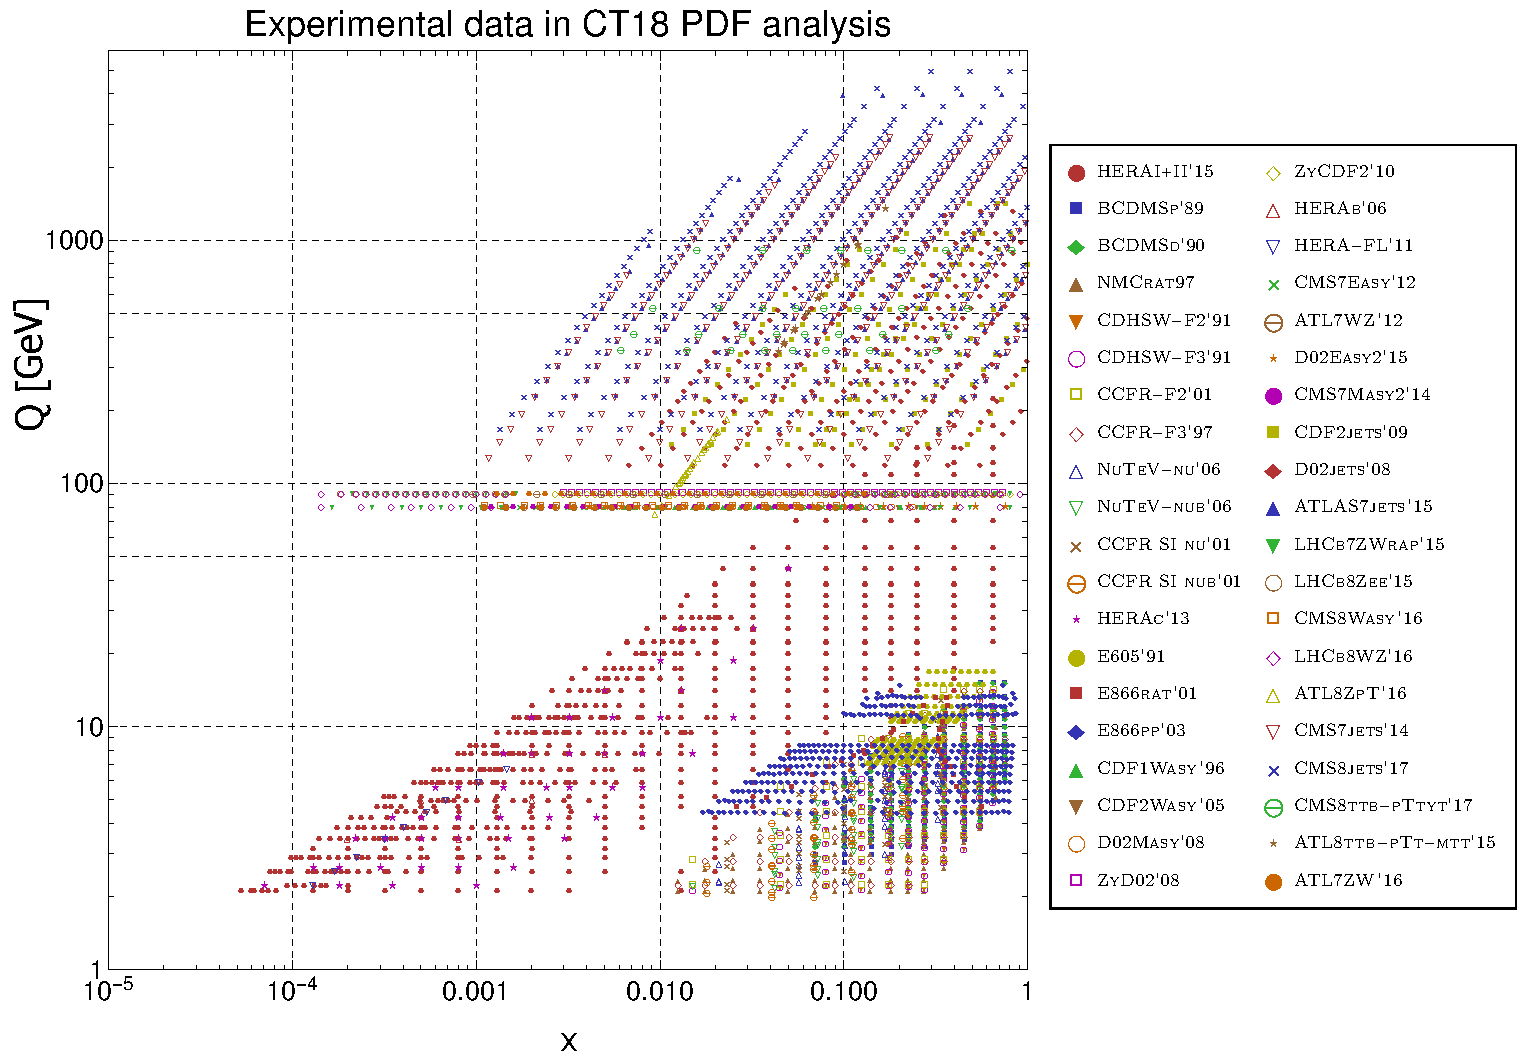
\includegraphics[width=0.99\textwidth]{./fig/ct18data_xmu.pdf}
	\caption{The CT18 data set, represented in a space of partonic $(x,\Q)$,
		based on Born-level kinematical matchings, $(x,\Q) = (x_B, Q)$, in DIS, {\it etc.}.
		The matching conventions used here are described in Ref.~\cite{Wang:2018heo}. Also
		shown are the ATLAS 7 TeV $W/Z$ production data (ID=248), labeled ATL7WZ'12, fitted
		in CT18Z.
		\label{fig:ct18data_xmu}}
\end{figure}

By 2018, the LHC collaborations published
about three dozen experimental data sets that can potentially constrain 
the CT PDFs. In light of the unprecedented precision reached in some 
measurements, the latest LHC data must be analyzed using
NNLO theoretical predictions in perturbative QCD.
%
The fitted PDFs we obtain in this analysis are plotted in Fig.~\ref{fig:ct18pdf},
which displays in the upper panels the CT18 PDFs at two widely-separated scales,
$\Q\!=\!2$ and $\,100$ GeV (on the left and right, respectively). In the lower panels,
we show the corresponding PDFs found in our amalgamated alternative analysis,
CT18Z.

%
\begin{figure}[htbp]
	\hspace*{-0.9cm}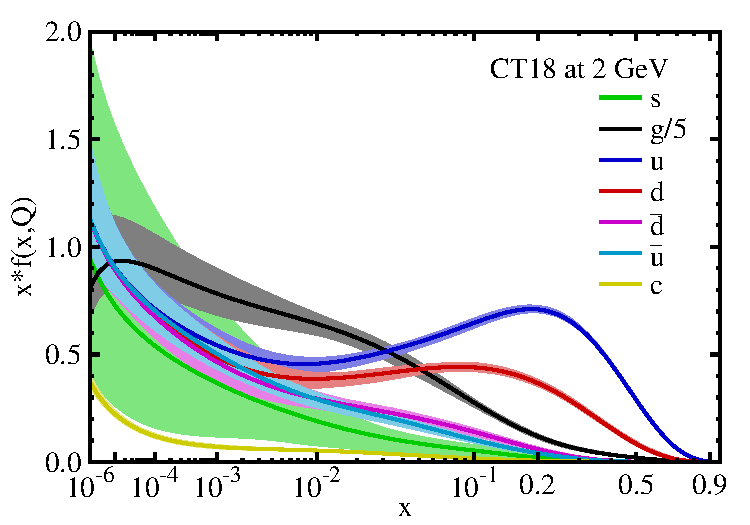
\includegraphics[width=0.52\textwidth]{./fig/pdfs_CT18___2GeV_Epdfs_cus-lin_ect.pdf}
	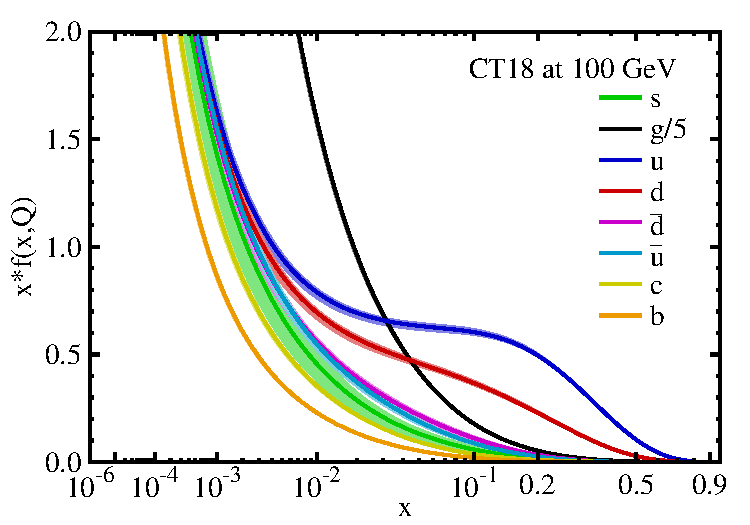
\includegraphics[width=0.52\textwidth]{./fig/pdfs_CT18_100GeV_Epdfs_cus-lin_ect.pdf}
	\hspace*{-0.9cm}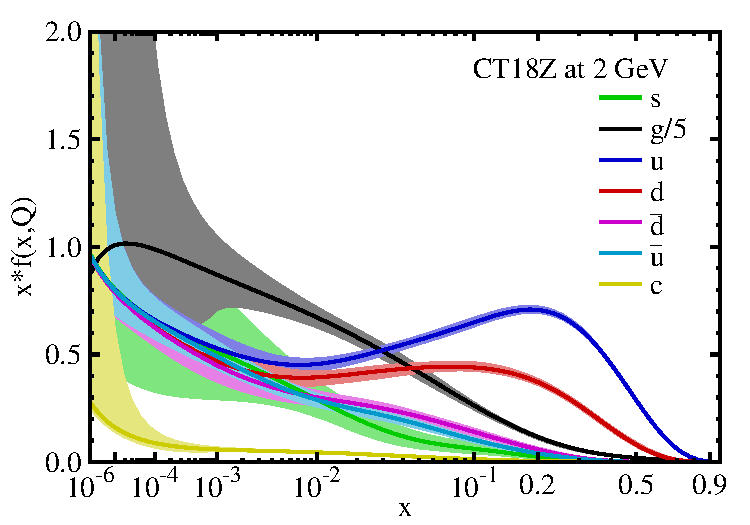
\includegraphics[width=0.52\textwidth]{./fig/pdfs_CT18ZNNLO___2GeV_A90CL_Epdfs_cus-lin-d5_ect.pdf}
	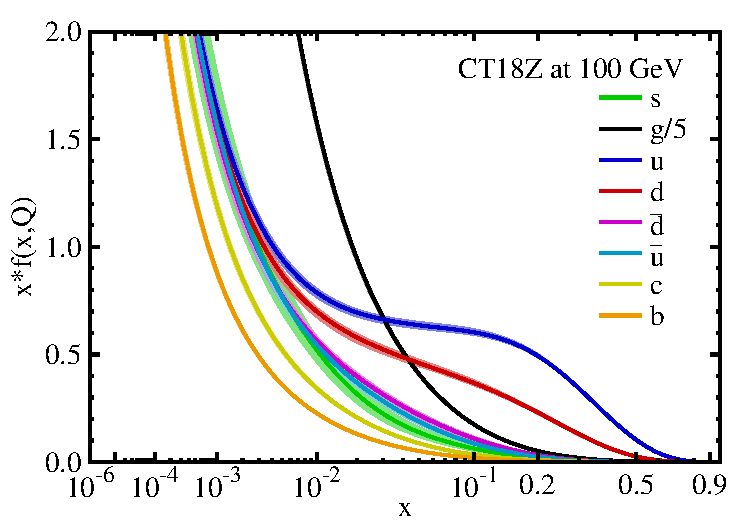
\includegraphics[width=0.52\textwidth]{./fig/pdfs_CT18ZNNLO_100GeV_A90CL_Epdfs_cus-lin-d5_ect.pdf}
	\caption{Upper panels: The CT18 parton distribution functions at $\Q\! =\! 2$ GeV and $\Q\! =\! 100$ GeV for
		$u, \overline{u}, d, \overline{d}, s = \overline{s}$, and $g$. 
		Lower panels: The analogous curves, but obtained for CT18Z. In all
		instances, the gluon PDF has been scaled down as $g(x,\Q)/5$.
		The charm distribution, $c(x,\Q)$, which
		is perturbatively generated by evolving from $Q_0\! =\! 1.3$ and 1.4 GeV, respectively, in CT18 and CT18Z, is also shown.
		\label{fig:ct18pdf}}
\end{figure}
%

Among the four ensembles (CT18, A, X, and Z) of PDFs,  the CT18 and CT18Z ensembles are the most dissimilar in terms of the shapes of PDFs, notably in the $x$ dependence of the fitted gluon and strangeness
distributions, $g(x,Q)$ and $s(x,\Q)$, as well as in some PDF uncertainties. For CT18, we obtain modest improvements in the precision
for the gluon density $g(x,\Q)$, as compared to CT14, following the inclusion of the LHC Run-1 data discussed below. For CT18Z, however, we obtain a somewhat enlarged uncertainty for the gluon and perturbatively-generated charm PDFs, especially at the lowest values
of $x\! <\! 10^{-3}$, due to the modified treatment of the DIS data described in
Sec.~\ref{sec:alt} and App.~\ref{sec:AppendixCT18Z}.
These final PDFs depend on numerous systematic factors in the experimental data. Scrupulous examination of the systematic effects was essential for trustworthy estimates of PDF uncertainties, 
and the scope of numerical computations also needed to be expanded. 

\subsubsection{\label{sec:summary-HERA2} Combined HERA I+II DIS data and the $x_B$-dependent factorization scale }
%
Even in the LHC era, DIS data from the $ep$ collider HERA provide the dominant
constraints on the CT18 PDFs. This dominance is revealed by independently applying the \texttt{ePump}, \texttt{PDFSense},  and Lagrange Multiplier methods.
CT18 implements the final (``combined'') data set from DIS at
HERA Run-I and Run-II \cite{Abramowicz:2015mha} that supersedes the HERA Run-I
only data set \cite{Aaron:2009aa} used in CT14 \cite{Dulat:2015mca}.
A transitional PDF set, \CTHERAII, was released based on fitting the
final HERA data \cite{Hou:2016nqm}. We found fair overall agreement of the HERA I+II
data with both CT14 and \CTHERAII~PDFs, and that both PDF ensembles
describe equally well the non-HERA data included in our global analysis.
At the same time, we observed some disagreement (``statistical tension'') 
between the $e^{+}p$ and $e^{-}p$ DIS cross sections of the HERA I+II data set. 
We determined that, at the moment, no plausible explanation could be provided to describe 
the full pattern of these tensions, as they are distributed across
the whole accessible range of Bjorken $x$ and lepton-proton momentum
transfer $Q$ at HERA.
%
%
Extending these studies using the CT18 fit, we have investigated the impact of the choice of
QCD scales on inclusive DIS data in the small-$x_B$ region, as will be explained later in
Sec.~\ref{sec:alt}.

\begin{figure}[tb]
	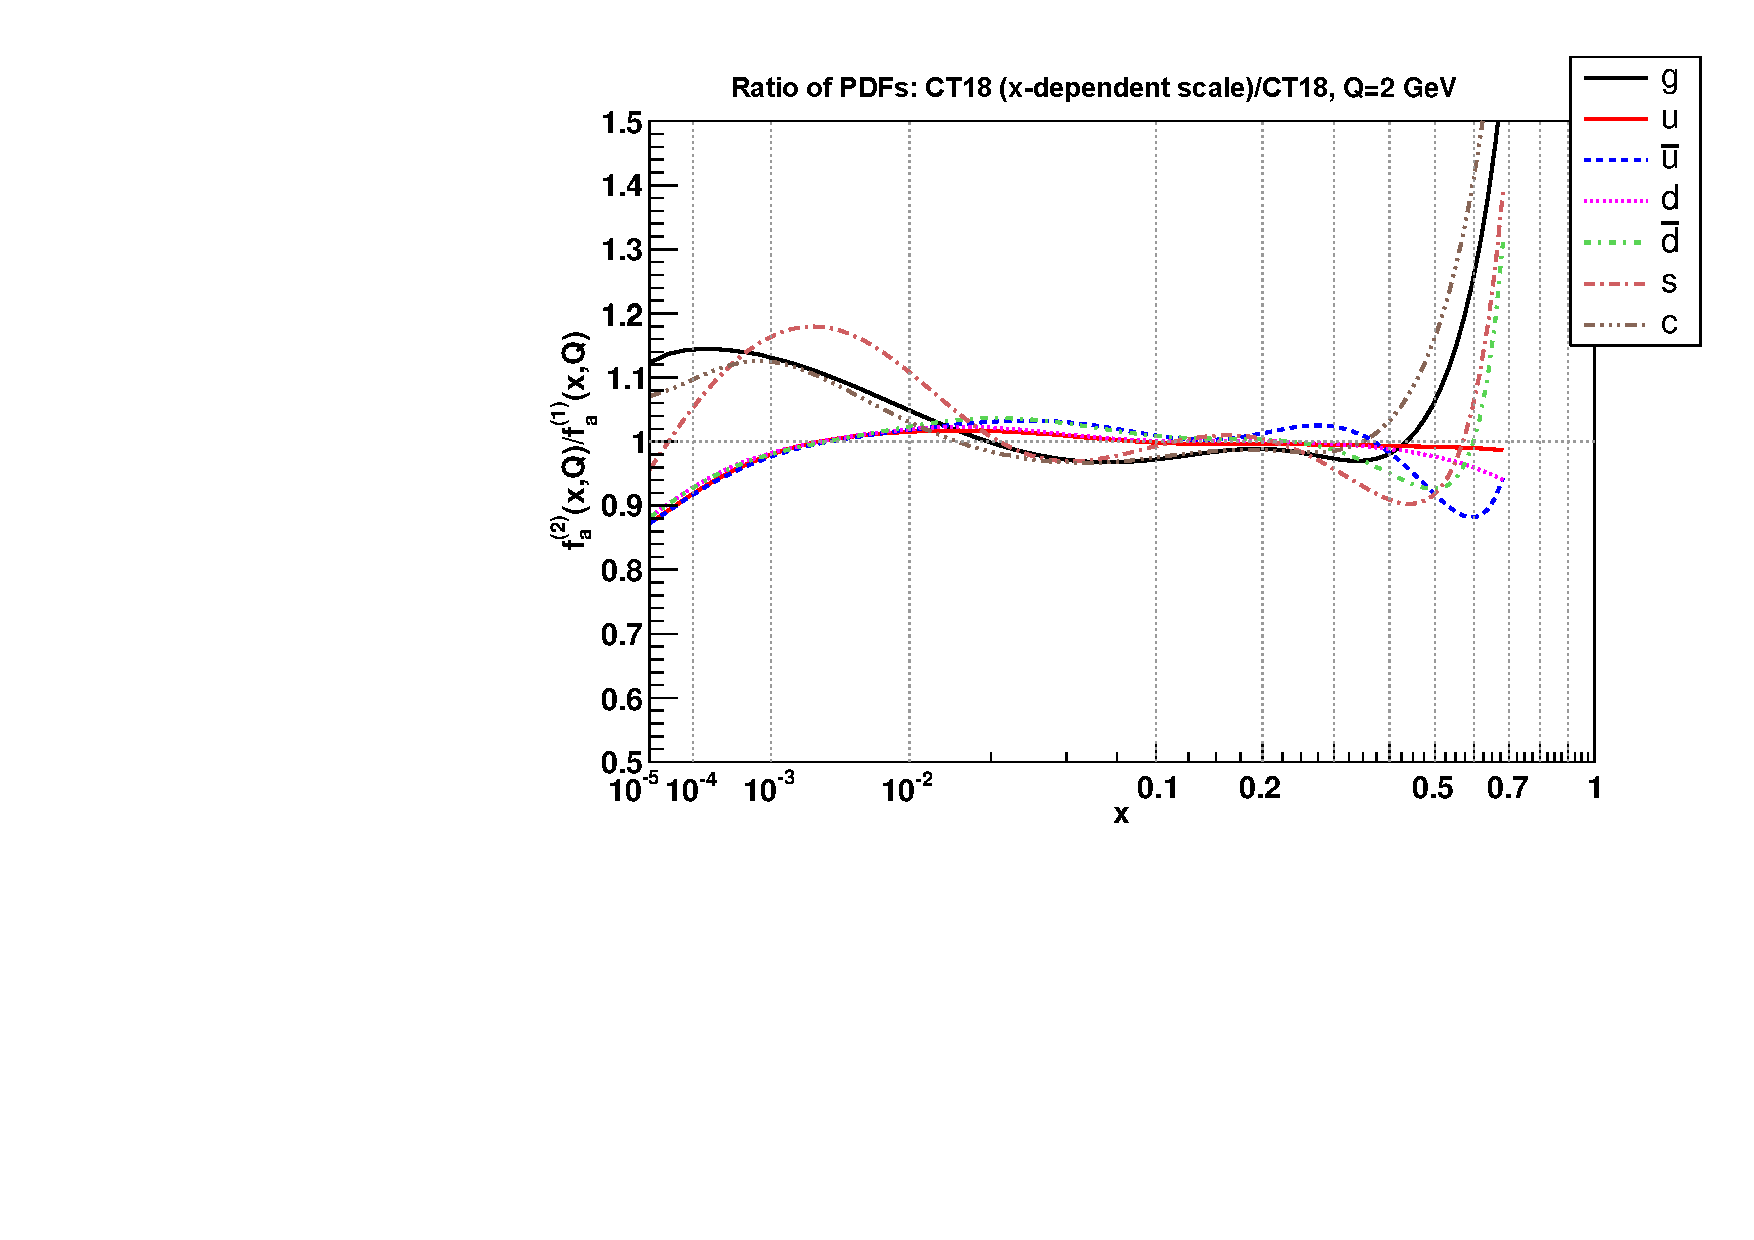
\includegraphics[width=0.59\textwidth]{./fig/ct18saturationToct18.pdf}
	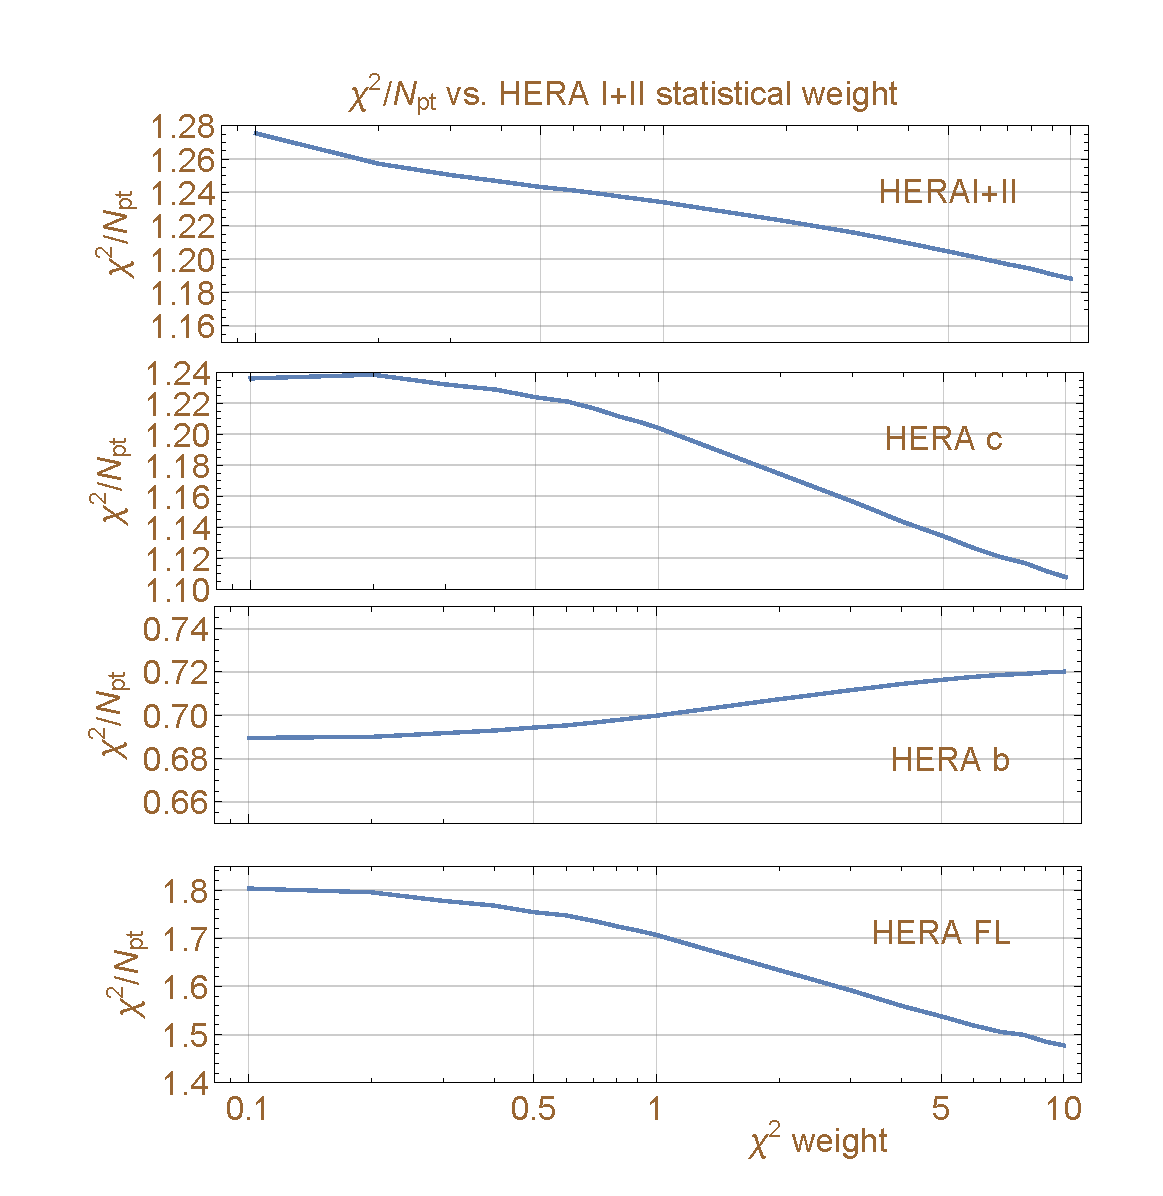
\includegraphics[width=0.4\textwidth]{./fig/HERAchi2NptWT_scan2Tct18z.pdf}
\caption{Left: The ratios of the candidate CT18 NNLO PDFs obtained with the
  $x_B$-dependent and standard factorization scales in DIS data
  sets. Right: The $\chi^2/N_{pt}$ values for four HERA data sets in
  the CT18Z fit with the $x_B$-dependent DIS factorization scale and
  varied statistical weight of the HERA I+II inclusive DIS data set.}
\label{fig:saturation}
\end{figure}


%
%
We find that the quality of fit to HERA data is improved by about 50 units by evaluating the NNLO theoretical cross sections in DIS with a special factorization scale, $\mu_{F,x}$, that depends on Bjorken $x_B$ (not the momentum fraction $x$) and is introduced in Section~\ref{sec:alt}. Fig.~\ref{fig:saturation} (left) shows
the changes in the candidate CT18 PDFs obtained by fitting the DIS data sets with the factorization scale $\mu_{F,x}$, as compared to the CT18 PDFs
with the nominal scale $\mu_F=Q$. With the scale $\mu_{F,x}$, we observe
reduced $u$ and $d$ (anti-)quark PDFs and increased gluon and
strangeness PDFs at $x < 10^{-2}$, as compared to the nominal CT18 fit,
with some compensating changes occurring in the same PDFs in the
unconstrained region $x > 0.5$ in order to satisfy the valence and
momentum sum rules. 

The right panel of Fig.~\ref{fig:saturation} shows the
$\chi^2/N_{pt}$ values ($\chi^2$ divided by the number, $N_\mathit{pt}$, of experimental data
points) for four HERA data sets (inclusive neutral and charged current DIS
\cite{Abramowicz:2015mha},
reduced charm, bottom production cross sections, and H1 longitudinal function
$F_L(x_B,Q^2)$ \cite{Collaboration:2010ry}) in the fits as a function of the
statistical weight $w$ of the HERA I+II inclusive DIS data set \cite{Abramowicz:2015mha}. The
default CT18Z fit corresponds to $w=1$; with $w=10$, the CT18Z fit
increasingly behaves as a HERA-only fit. We see that, with the scale
$\mu^2_{F,x}$ and $w=10$, $\chi^2/N_{pt}$ for the inclusive DIS data set
improves almost to the levels observed in the ``resummed'' HERA-only fits
without intrinsic charm \cite{Ball:2017otu,Abdolmaleki:2018jln}. The
quality of the fit to the charm semi-inclusive DIS (SIDIS) cross section and H1 $F_L$ also improves.

The new combined charm and bottom production measurements from the H1 and Zeus collaborations published in Ref.~\cite{H1:2018flt} (2018) have been investigated and in their current version, when these measurements replace the previous ones in the CT18 global analysis, they cannot be fitted with a reasonable $\chi^2$.
Moreover, a mild tension is observed between these new combined data and several CT18 data sets such as the LHCb 7 and 8 TeV $W/Z$ production data, $Z$-rapidity data at CDF run II, CMS 8 TeV single inclusive jet production, and $t\bar{t}$ double differential $p_T$ and $y$ cross section. Therefore, we decided not to include these data in the CT18 global analysis as they require a dedicated investigation.
In the H1+ZEUS analysis of Ref.~\cite{H1:2018flt}, the $\chi^2$ for these measurements is also found not to be optimal. This is ascribed to a difference in the slope between data and theory in the intermediate/small $x$ region. In our attempt to fit the new combined charm and bottom production measurements, we have noticed a preference for a harder gluon at intermediate/small $x$.
We are currently investigating these data separately and, in particular, we are exploring the impact of the new correlated systematic uncertainties as they increased from 42 in the old version of the data, to 167 in the new version.
The results of this new study are going to be published in a separate forthcoming paper.



\begin{figure}[tb]
	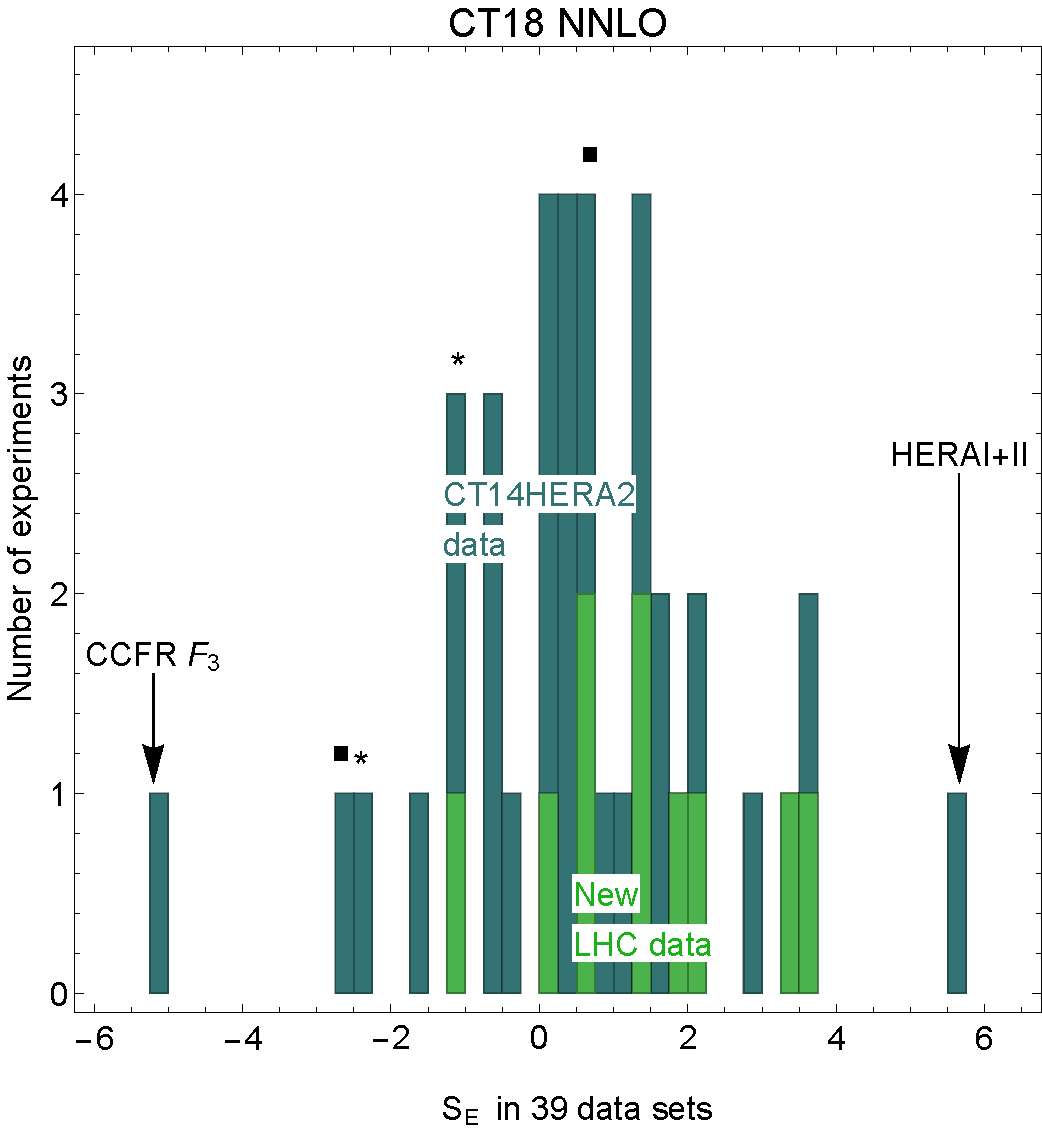
\includegraphics[width=0.6\textwidth]{./fig/sqrt2chi2_ct18nnloCount.pdf}
	\caption{A histogram of the effective Gaussian variable ($S_E$) distributed over all CT18 data sets. 
	Two squares and two stars indicate the $S_E$ values for the NuTeV dimuon and CCFR dimuon data, respectively.
\label{fig:sn_ct18}}
\end{figure}

\subsubsection{Selection of new LHC experiments \label{sec:ExptSelection} }
When selecting the 
most promising LHC experiments for the CT18 fit, 
we had to address a recurrent challenge --- the presence of statistical
tensions among various (sub)sets of the latest experimental data from
HERA, LHC, and the Tevatron. The quickly improving precision of the collider
data reveals previously irrelevant anomalies either in the experiment
or theory. These anomalies are revealed by applying strong goodness-of-fit
tests~\cite{Kovarik:2019xvh}. Figure~\ref{fig:sn_ct18}
illustrates the degree of tensions using a representation based on the effective
Gaussian variables $S_E\equiv \sqrt{2\chi_E^2}-\sqrt{2 N_E-1}$~\cite{Lai:2010vv}
constructed from the $\chi^2$ values and numbers of data points $N_\mathit{E}$ for
individual data sets $E$. In an ideal fit in which the differences between theory and data are consistent with Gaussian random fluctuations, the probability
distribution for $S_E$ must be approximately a standard normal
distribution (with a unit half-width). In the global fits by CTEQ-TEA and  external groups, we rather observe wider $S_E$ distributions
as in Fig.~\ref{fig:sn_ct18}, with some of the more comprehensive
and precise data sets (notably, HERA I+II inclusive DIS
\cite{Abramowicz:2015mha} and ATLAS 7 TeV $W/Z$ production
\cite{Aaboud:2016btc}) having $S_E$ values as high as five units or more.  
The question, then, is how to select clean and accurate experiments for
the global analysis from an ever-growing list of measurements, while
maximally preserving the consistency of the selected experiments. 
For example, there are many LHC data sets~\cite{Rojo:2015acz}
that are potentially sensitive to the PDFs, including novel measurements
involving the production of high-$p_{T}$ $Z$ bosons, $t\bar{t}$ pairs,
isolated photon, and small-$x$ heavy flavor (charm or bottom) quarks.
Including all such candidate experiments
into the full global fit is impractical: CPU costs grow quickly with
the number of experimental data sets at NNLO. Poorly fitted experiments
would increase, not decrease, the final PDF uncertainty. The generation
of one error PDF set took several days of CPU time in the CT14 fit
to 33 experiments in single-thread mode. Adding 20-30 additional
experiments with this setup was thus impossible.
The CTEQ-TEA group resolved
these challenges through a multi-pronged effort that allowed us
to include eleven new LHC data sets at 7 and 8 TeV on $W^\pm$, $Z$, jet, and $t\bar{t}$ production. 


\subsubsection{Advances in fitting methodology \label{sec:Advances} }
To identify the eligible experimental
data sets for the global fit, we developed two programs for fast preliminary analysis. The \texttt{PDFSense} program~\cite{Wang:2018heo} 
was developed at Southern Methodist University (SMU)
to predict quantitatively, and before doing the fit, which data sets
will have an impact on the global PDF fit. The \texttt{ePump} program~\cite{Schmidt:2018hvu} 
developed at Michigan State University (MSU)
applies Hessian profiling to quickly estimate the impact of data on the
PDFs prior to the global fit. These programs provide helpful guidelines
for the selection of the most valuable experiments based entirely on the previously published Hessian error PDFs.

 As we will discuss in Appendix~\ref{sec:Appendix4xFitter}, the out-of-the-box algorithm for Hessian profiling implemented in the 
 commonly used version 2.0.0 of the \texttt{xFitter} program~\cite{Bertone:2016ywq} is inconsistent with the CTEQ-TEA definitions 
 of PDF uncertainties and has predicted  too optimistic $\chi^2$ values and PDF uncertainties in a number 
 of studies for profiling the CTEQ-TEA PDFs. The \texttt{ePump} program does not have this caveat. 
 Its Hessian updating algorithm better reproduces the $\chi^2$ values of the data sets in the full CT14 and CT18 fits, 
 as well as the respective PDF uncertainties defined according to the two-tier definition of $\chi^2$ adopted in the CTEQ-TEA analyses since CT10 NLO~\cite{CT10NNLO}. 

The CTEQ fitting code was parallelized to allow a faster turnaround
time (one fit within a few hours instead of many days) on high-performance
computing clusters. For as much relevant LHC data as possible, we computed
the NLO cross sections with the \texttt{APPLGrid/fastNLO} tables~\cite{Kluge:2006xs,Carli:2010rw}  (to be multiplied by tabulated point-by-point NNLO/NLO $K$-factor corrections)
for various new LHC processes: production of $W/Z$ bosons, high-$p_{T}$
$Z$-bosons and inclusive jets; the NNLO cross section with the \texttt{fastNNLO} tables \cite{Czakon:2017dip,fastnnlo:grids} for the $t\bar{t}$ pair production at the LHC. The \texttt{APPLgrid} tables were cross validated
against similar tables from other groups (available in the public
domain) and optimized for speed and accuracy. 

\subsubsection{Estimates of theoretical and parametrization uncertainties}
Significant effort was spent on understanding the sources
of PDF uncertainties. Theoretical uncertainties associated with the
scale choice were investigated for the affected processes, such as
DIS as well as inclusive jet and high-$p_{T}$ $Z$ boson production. Other considered theoretical uncertainties were due 
to the differences among the NNLO/resummation codes ({\it e.g.}, \texttt{DYNNLO}~\cite{Catani:2007vq,Catani:2009sm}, 
\texttt{MCFM}~\cite{Campbell:2010ff, Boughezal:2016wmq, MCFM8}, 
\texttt{FEWZ}~\cite{Gavin:2010az, Gavin:2012sy, Li:2012wna},
\texttt{ResBos}~\cite{Ladinsky:1993zn, Balazs:1997xd}
and \texttt{NNLOJet}~\cite{Ridder:2015dxa,Gehrmann-DeRidder:2017mvr,Currie:2016bfm,Currie:2017ctp}) and Monte-Carlo (MC) integration error, see Sec.~\ref{sec:calcs}.
The important PDF parametrization uncertainty was investigated by repeating
the fits for $\mathcal{O}(100)$ trial functional forms of the PDFs. [Our post-CT10
fits parametrize PDFs in terms of Bernstein polynomials, which simplify
trying a wide range of parametrization forms to quantify/eliminate
potential biases. Appendix~\ref{sec:AppendixParam} presents an example of such parametrization.]

\subsubsection{General-purpose and specialized PDFs \label{sec:General-purpose}}
The final CT18(Z) data ensemble contains a total of $N_\mathit{pt}\! =\! 3681(3493)$ data points and results in $\chi^2/N_\mathit{pt}=1.17 (1.19)$ at NNLO.
The four families of {\it general-purpose} CT18 PDFs presented in this paper are most suitable for computations of central predictions and estimations of PDF uncertainties in accord with the guidelines on the usage of PDFs published by the PDF4LHC group \cite{Butterworth:2015oua}. The PDF uncertainties are constructed at the 90\% probability level based on two tiers of criteria as in the CT14 global analysis \cite{Dulat:2015mca}.  These PDFs are obtained by assuming a world-average QCD coupling constant, $\alpha_s(M_Z)=0.118$ \cite{Tanabashi:2018oca}. The combined PDF+$\alpha_s$ uncertainty can be computed using the special $\alpha_s$ series of the PDFs for each family by adding the PDF and $\alpha_s$ uncertainties in quadrature, as explained in Ref.~\cite{Lai:2010nw}.

As we have done with the previous families of the CTEQ-TEA PDFs, we intend to produce specialized PDF sets to complement the current general-purpose PDF ensembles. In particular, CT18 updates on the PDFs with an asymmetric-strangeness PDF~ \cite{Lai:2007dq}, photon PDF \cite{Schmidt:2015zda} and fitted charm \cite{Hou:2017khm} will be provided in future publications. 

\subsection{Experimental data sets fitted in CT18}
\label{sec:data_overview}

The CT18 global analysis starts with the data set baseline of \CTHERAII~\cite{Hou:2016nqm} and adds the latest precision LHC results. The experiments in the \CTHERAII~baseline
are listed in Table \ref{tab:EXP_1}, while the new LHC data sets included in the CT18(Z) fit are shown in Table \ref{tab:EXP_2}. 
Tables~\ref{tab:EXP_1} and~\ref{tab:EXP_2}
also include information on the number of data points, $\chi^2$, and the effective Gaussian variable, $S_E$, for each individual data set appearing in the global fit.   
%The impact of the new LHC measurements has been examined by adding  data sets one by one on top of the \CTHERAII ~baseline.  
%CRS - Sentenced moved to ePump section.
%
Most of the data sets are included in all four PDF ensembles; we  will identify differences between the specific selections as they arise.
%

\subsubsection{Charting sensitivity of new data sets to the PDFs \label{sec:Sensitivity} }

As discussed in Secs.~\ref{sec:ExptSelection} and \ref{sec:Advances}, we employed a new method based on the Hessian sensitivity variables \cite{Wang:2018heo,Hobbs:2019gob} ( informative descendants of the Hessian correlation between theoretical observables and PDFs~\cite{Pumplin:2001ct,Nadolsky:2001yg,Nadolsky:2008zw}) 
to determine quantitatively a hierarchy of impact of data on the global fit, and on specific cross sections. 

\begin{figure}[tb]
	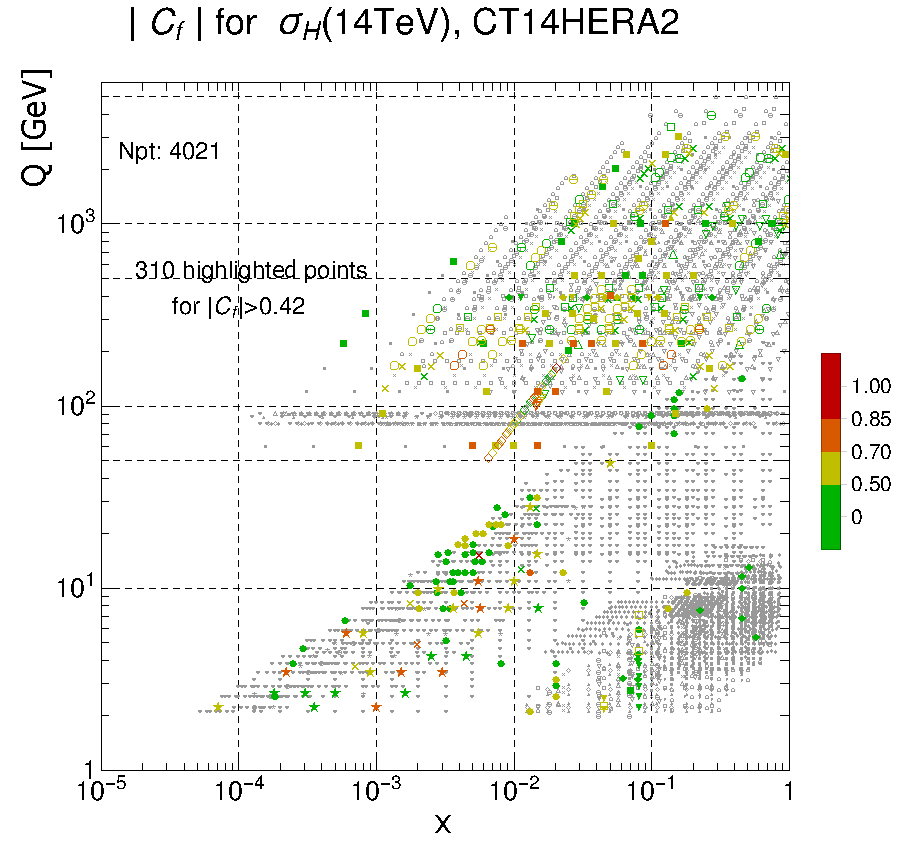
\includegraphics[width=0.48\textwidth]{./fig/Cf_higgs.pdf}
	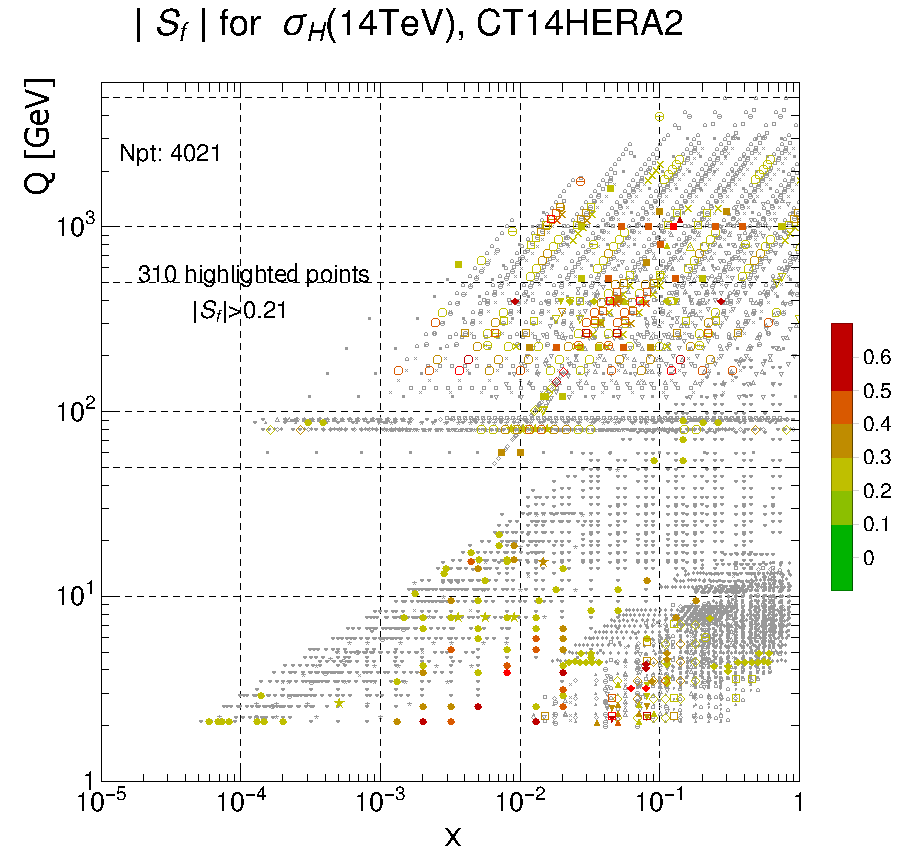
\includegraphics[width=0.48\textwidth]{./fig/Sf_higgs.pdf}
\caption{
	Left: Candidate data considered for inclusion in CT18
	evaluated according to the magnitude of the Pearson
	correlation $C_f$ between the total Higgs cross section at 14 TeV,
	$\sigma_{H}(14\, \mathrm{TeV})$ and the residual of
	each point as determined within the \texttt{PDFSense}
	framework~\cite{Wang:2018heo}.
	Right: A similar assessment of the CT18 candidate data,
	but computed on the basis of the {\it sensitivity},
	$|S_f|(x_i,\Q_i)$. In both panels, a highlighting
	cut has been imposed to draw attention to the $\sim\!300$
	highest-impact points according to each metric.
  }
\label{fig:PDFSense}
\end{figure}

As a demonstration of this, the \texttt{PDFSense} framework can predict in advance which fitted data sets may have the most impact on one of the most crucial predictions at the LHC, such as the Higgs boson cross section ($\sigma_H$) through the $gg$ fusion process (at $\sqrt{s}=14$ TeV). Often, to get an indication which data sets will have the most impact on such cross sections, one examines the Pearson correlations \cite{Pumplin:2001ct,Nadolsky:2001yg,Nadolsky:2008zw} between the experimental data points and the gluon distribution in the kinematic region responsible for Higgs boson production.  The
left-hand side of Fig.~\ref{fig:PDFSense} shows the data points with the highest absolute correlations $|C_f|$ (defined by the statistical residuals as in Ref.~\cite{Wang:2018heo}) with the Higgs boson cross section at 14 TeV. 

By this measure, there may be a number of high-impact data sets, notably HERA neutral current DIS, LHC and Tevatron jet production, and HERA charm quark production.
The correlations, however, do not reflect the experimental uncertainties of the data points: an experimental cross section could be highly correlated with the gluon distribution in the $x$ range  responsible for Higgs boson production and still not provide much of a constraint
on the Higgs boson cross section if the experimental uncertainties are large. Conversely, an experimental cross section that might not have as large a correlation, but which has smaller (statistical and systematic) uncertainties,
may provide a stronger
constraint. 

The level of constraint is thus better predicted by the sensitivity variable $S_f$, defined in Ref.~\cite{Wang:2018heo}. The experimental data points used in the CT18 global fit that have the
highest absolute sensitivity $|S_f|$ to the PDF dependence of $\sigma_H$ at 14 TeV are shown on the right-hand side of Fig.~\ref{fig:PDFSense}. More data points (from a larger number of experiments) have high sensitivity
than those identified by high correlation. In addition to the DIS data from HERA I+II, there are also contributions from the fixed-target DIS experiments, as well as measurements from the LHC. 

As will be shown in Sec.~\ref{sec:LMScans} using Lagrange Multiplier scans, the HERA I+II data set, with its abundant data points and small experimental errors, 
still dominates the constraints on the gluon distribution in the range sensitive to Higgs boson production at the LHC. 
Because of the continuing influence of the older data sets, we will find that the reduction of the PDF uncertainty for Higgs boson production is less significant in CT18 than in CT14. In addition, tension between some of the most sensitive data sets limits the reduction on the uncertainty
of the Higgs cross section. These effects are explored in detail in Sec.~\ref{sec:LMScans}.

We will now discuss the new data sets included in the CT18 analysis, and highlight the differences in the alternative fits.


\subsubsection{Baseline data sets \label{sec:Baseline}}

The CT18 global analysis inherits from \CTHERAII~a number of precision non-LHC experiments listed in Table 1. Among those, the 
HERA I+II DIS data set provides the most significant constraints, followed by a group of fixed-target neutral-current DIS experiments: BCDMS, NMC, and CCFR.
Similarly, a number of neutrino DIS measurements have previously been included
and provide valuable constraints on sea (anti-)quarks.
Among them, we find that the single-nucleon structure functions $F_2^p$ and $F_3^p$ extracted from CDHSW data on neutrino-iron 
deep inelastic scattering exhibit a preference for a harder gluon PDF at $x \gtrsim 0.1$, compared to CCFR and other experiments, cf. Fig.~\ref{fig:LMg18}. 
This well-known behavior reflects  larger logarithmic slopes of $F_2^p$ and $x F_3^p$ measured by CDHSW, as compared to the 
analogous CCFR measurements~\cite{Seligman:1997fe}, which in turn may reflect differences in the energy calibration and resolution smearing between the two experiments~\cite{Bodek:1996zu}. 
Thus, to help obtain a softer large-$x$ gluon behavior, as being favored by recent LHC data, we exclude the CDHSW $F_2$ and $x_B F_3$ data sets from the CT18Z analysis, while including these sets in the rest of the CT18 PDF ensembles. 

We continue to include a variety of lepton pair production measurements from the Tevatron and fixed-target 
experiments, as summarized in Table~\ref{tab:EXP_1}. The low-statistics data on $W/Z$ production at 
LHCb 7 TeV~\cite{Aaij:2012vn} and ATLAS, CMS 7 TeV jet production \cite{Aad:2011fc, Chatrchyan:2012bja} 
are replaced in the CT18 analyses by more recent measurements, as summarized in the next section. 

\begin{widetext}

\begingroup
\squeezetable
\begin{table}[htbp]
\begin{tabular}{|l|lr|c|c|c|c|}
\hline
\textbf{ID\# }  & \textbf{Experimental data set} &  & $N_{pt, E}$  & $\chi^2_E$ & $\chi^{2}_E/N_{pt, E}$  & $S_E$ \tabularnewline
\hline
\hline
%
 160 & HERAI+II 1 fb$^{-1}$, H1 and ZEUS NC and CC $e^\pm p$ reduced cross sec. comb.      & \cite{Abramowicz:2015mha}   & 1120  &  1408(1378) &   1.3( 1.2) &   5.7(  5.1)   \tabularnewline\hline
 101 & BCDMS $F_{2}^{p}$                                                                   & \cite{Benvenuti:1989rh}     &  337  &   374 ( 384) &   1.1( 1.1) &   1.4(  1.8)   \tabularnewline\hline
 102 & BCDMS $F_{2}^{d}$                                                                   & \cite{Benvenuti:1989fm}     &  250  &   280 ( 287) &   1.1( 1.1) &   1.3(  1.6)   \tabularnewline\hline
 104 & NMC $F_{2}^{d}/F_{2}^{p}$                                                           & \cite{Arneodo:1996qe}       &  123  &   126 ( 116) &   1.0( 0.9) &   0.2( -0.4)   \tabularnewline\hline
 108$^{\dagger}$ & CDHSW $F_{2}^{p}$                                                       & \cite{Berge:1989hr}         &   85  &    85.6 ( 86.8) &   1.0( 1.0) &   0.1(  0.2)   \tabularnewline\hline         
 109$^{\dagger}$ & CDHSW $x_B F_{3}^{p}$                                                       & \cite{Berge:1989hr}         &   96  &    86.5 (  85.6) &   0.9( 0.9) &  -0.7( -0.7)   \tabularnewline\hline
 110 & CCFR $F_{2}^{p}$                                                                    & \cite{Yang:2000ju}          &   69  &    78.8(  76.0) &   1.1( 1.1) &   0.9(  0.6)   \tabularnewline\hline
 111 & CCFR $x_B F_{3}^{p}$                                                                   & \cite{Seligman:1997mc}      &   86  &    33.8(  31.4) &   0.4( 0.4) &  -5.2( -5.6)   \tabularnewline\hline
 124 & NuTeV $\nu\mu\mu$ SIDIS                                                             & \cite{Mason:2006qa}         &   38  &    18.5(  30.3) &   0.5( 0.8) &  -2.7( -0.9)   \tabularnewline\hline
 125 & NuTeV $\bar\nu \mu\mu$ SIDIS                                                        & \cite{Mason:2006qa}         &   33  &    38.5(  56.7) &   1.2( 1.7) &   0.7(  2.5)   \tabularnewline\hline
 126 & CCFR $\nu\mu\mu$ SIDIS                                                              & \cite{Goncharov:2001qe}     &   40  &    29.9(  35.0) &   0.7( 0.9) &  -1.1( -0.5)   \tabularnewline\hline
 127 & CCFR  $\bar\nu \mu\mu$ SIDIS                                                        & \cite{Goncharov:2001qe}     &   38  &    19.8(  18.7) &   0.5( 0.5) &  -2.5( -2.7)   \tabularnewline\hline
 145 & H1 $\sigma_{r}^{b}$                                                                 & \cite{Aktas:2004az}         &   10  &     6.8(   7.0) &   0.7( 0.7) &  -0.6( -0.6)   \tabularnewline\hline
 147 & Combined HERA charm production                                                      & \cite{Abramowicz:1900rp}    &   47  &    58.3(  56.4) &   1.2( 1.2) &   1.1(  1.0)   \tabularnewline\hline
 169 & H1 $F_{L}$                                                                          & \cite{Collaboration:2010ry} &    9  &    17.0(  15.4) &   1.9( 1.7) &   1.7(  1.4)   \tabularnewline\hline
 201 & E605 Drell-Yan process                                                              & \cite{Moreno:1990sf}        &  119  &   103.4( 102.4) &   0.9( 0.9) &  -1.0( -1.1)   \tabularnewline\hline
 203 & E866 Drell-Yan process  $\sigma_{pd}/(2\sigma_{pp})$                                & \cite{Towell:2001nh}        &   15  &    16.1(  17.9) &   1.1( 1.2) &   0.3(  0.6)   \tabularnewline\hline
 204 & E866 Drell-Yan process  $Q^3 d^2\sigma_{pp}/(dQ dx_F)$                              & \cite{Webb:2003ps}          &  184  &   244 ( 240) &   1.3( 1.3) &   2.9(  2.7)   \tabularnewline\hline
 225 & CDF Run-1 electron  $A_{ch}$, $p_{T\ell}>25$ GeV                                    & \cite{Abe:1996us}           &   11  &     9.0(   9.3) &   0.8( 0.8) &  -0.3( -0.2)   \tabularnewline\hline
 227 & CDF Run-2 electron $A_{ch}$, $p_{T\ell}>25$ GeV                                     & \cite{Acosta:2005ud}        &   11  &    13.5(  13.4) &   1.2( 1.2) &   0.6(  0.6)   \tabularnewline\hline
 234 & D\O~ Run-2 muon $A_{ch}$, $p_{T\ell}>20$ GeV                                        & \cite{Abazov:2007pm}        &    9  &     9.1(   9.0) &   1.0( 1.0) &   0.2(  0.1)   \tabularnewline\hline
 260 & D\O~ Run-2 $Z$ rapidity                                                             & \cite{Abazov:2006gs}        &   28  &    16.9(  18.7) &   0.6( 0.7) &  -1.7( -1.3)   \tabularnewline\hline
 261 & CDF Run-2 $Z$ rapidity                                                              & \cite{Aaltonen:2010zza}     &   29  &    48.7(  61.1) &   1.7( 2.1) &   2.2(  3.3)   \tabularnewline\hline
 266 & CMS 7 TeV $4.7\mbox{ fb}^{-1}$, muon $A_{ch}$, $p_{T\ell}>35$ GeV                   & \cite{Chatrchyan:2013mza}   &   11  &     7.9(  12.2) &   0.7( 1.1) &  -0.6(  0.4)   \tabularnewline\hline
 267 & CMS 7 TeV $840\mbox{ pb}^{-1}$, electron $A_{ch}$, $p_{T\ell}>35$ GeV               & \cite{Chatrchyan:2012xt}    &   11  &    11.8(  16.1) &   1.1( 1.5) &   0.3(  1.1)   \tabularnewline\hline
 268$^{\ddagger\ddagger}$ & ATLAS 7 TeV $35\mbox{ pb}^{-1}$ $W/Z$ cross sec., $A_{ch}$                          & \cite{Aad:2011dm}           &   41  &    44.4   (50.6) &   1.1( 1.2) &   0.4(  1.1)   \tabularnewline\hline
 281 & D\O~ Run-2 $9.7 \mbox{ fb}^{-1}$ electron $A_{ch}$, $p_{T\ell}>25$ GeV              & \cite{D0:2014kma}           &   13  &    22.8(  20.5) &   1.8( 1.6) &   1.7(  1.4)   \tabularnewline\hline
 504 & CDF Run-2 inclusive jet production                                                  & \cite{Aaltonen:2008eq}      &   72  &   122 ( 117) &   1.7( 1.6) &   3.5(  3.2)   \tabularnewline\hline
 514 & D\O~ Run-2 inclusive jet production                                                 & \cite{Abazov:2008ae}        &  110  &   113.8 ( 115.2) &   1.0( 1.0) &   0.3(  0.4)   \tabularnewline
\hline
\hline
\end{tabular}
\caption{Data sets included in the CT18(Z) NNLO global analyses. Here we directly compare the quality-of-fit found for CT18 NNLO vs.~CT18Z NNLO on the basis of $\chi^2_E$,
	$\chi^2_E/N_{pt, E}$, and $S_E$, in which $N_{pt, E}$, $\chi^2_E$ are the number of points and value of $\chi^2$ for  experiment  $E$ at the global minimum. $S_E$ is
	the effective Gaussian parameter \cite{Lai:2010vv, Gao:2013xoa, Dulat:2013hea} quantifying agreement with each experiment. The ATLAS 7 TeV $35\mbox{ pb}^{-1}$ $W/Z$ data set, marked
	by $\ddagger\ddagger$, is replaced by the updated one (4.6 fb$^{-1}$) in the CT18A and CT18Z fits. The CDHSW data, labeled by $\dagger$, are not included in the CT18Z fit. The numbers in parentheses are for the CT18Z NNLO fit.
\label{tab:EXP_1} }
\end{table}
\endgroup
\end{widetext}

\begin{widetext}
\begingroup
\squeezetable
\begin{table}[tb]
\begin{tabular}{|l|lr|c|c|c|c|}
\hline
\textbf{ID\# }  & \textbf{Experimental data set} &  & $N_{pt, E}$  & $\chi^2_E$ & $\chi^{2}_E/N_{pt, E}$  & $S_E$ \tabularnewline
\hline
\hline
 245 & LHCb 7 TeV 1.0 fb$^{-1}$ $W/Z$ forward rapidity cross sec.                          & \cite{Aaij:2015gna}        &  33  &   53.8 (  39.9) &  1.6 (  1.2) &  2.2 ( 0.9) \tabularnewline\hline
 246 & LHCb 8 TeV  2.0 fb$^{-1}$ $Z\rightarrow e^{-} e^{+}$ forward rapidity cross sec.    & \cite{Aaij:2015vua}        &  17  &   17.7 (  18.0) &  1.0 (  1.1) &  0.2 ( 0.3) \tabularnewline\hline
 248$^{\ddagger}$ & ATLAS 7 TeV 4.6 fb$^{-1}$, $W/Z$ combined cross sec.                   & \cite{Aaboud:2016btc}      &  34  &  287.3 (  88.7) &  8.4 (  2.6) & 13.7 ( 4.8) \tabularnewline\hline
 249 & CMS 8 TeV 18.8 fb$^{-1}$ muon charge asymmetry $A_{ch}$                                & \cite{Khachatryan:2016pev} &  11  &   11.4 (  12.1) &  1.0 (  1.1) &  0.2 ( 0.4) \tabularnewline\hline
 250 & LHCb 8 TeV 2.0fb$^{-1}$ $W/Z$ cross sec.                                            & \cite{Aaij:2015zlq}        &  34  &   73.7 (  59.4) &  2.1 (  1.7) &  3.7 ( 2.6) \tabularnewline\hline 
% 251 & ATLAS 8 TeV 20.3 fb$^{-1}$ single diff. high-mass cross sec.                        & \cite{Aad:2016zzw}         &  12  &   20.4 (  16.3) &  1.7 (  1.4) &  1.7 ( 0.9) \tabularnewline\hline
 253 & ATLAS 8 TeV 20.3 fb$^{-1}$, $Z$ $p_T$ cross sec.                                    & \cite{Aad:2015auj}         &  27  &   30.2 (  28.3) &  1.1 (  1.0) &  0.5 ( 0.3) \tabularnewline\hline
 542 & CMS 7 TeV 5 fb$^{-1}$, single incl. jet cross sec., $R=0.7$ (extended in y)         & \cite{Chatrchyan:2014gia}  & 158  &  194.7 ( 188.6) &  1.2 (  1.2) &  2.0 ( 1.7) \tabularnewline\hline
 544 & ATLAS 7 TeV  4.5 fb$^{-1}$, single incl. jet cross sec., $R=0.6$                    & \cite{Aad:2014vwa}         & 140  &  202.7 ( 203.0) &  1.4 (  1.5) &  3.3 ( 3.4) \tabularnewline\hline
 545 & CMS 8 TeV 19.7 fb$^{-1}$, single incl. jet cross sec., $R=0.7$, (extended in y)     & \cite{Khachatryan:2016mlc} & 185  &  210.3 ( 207.6) &  1.1 (  1.1) &  1.3 ( 1.2) \tabularnewline\hline
 573 & CMS 8 TeV 19.7 fb$^{-1}$, $t\bar{t}$ norm. double-diff. top $p_T$ and $y$ cross sec. & \cite{Sirunyan:2017azo}    &  16  &   18.9 (  19.1) &  1.2 (  1.2) &  0.6 ( 0.6) \tabularnewline\hline
 580 & ATLAS 8 TeV 20.3$^{-1}$, $t\bar{t}$ $p_{T}^{t}$ and $m_{t\bar{t}}$ abs. spectrum    & \cite{Aad:2015mbv}         &  15  &    9.4 (  10.7) &  0.6 (  0.7) & -1.1 (-0.8) \tabularnewline
 \hline
\end{tabular}
\caption{Like Table~\ref{tab:EXP_1}, for newly-included LHC measurements.
	The ATLAS 7 TeV $W/Z$ data (4.6 fb$^{-1}$), labeled by $\ddagger$, are included in the CT18A and CT18Z global fits, but not in CT18 and CT18X. 
	%Similarly, the ATLAS 7 TeV $35\mbox{ pb}^{-1}$ $W/Z$ cross section data, marked by $\ddagger\ddagger$, are not fitted in CT18A and CT18Z.  
    %The CDHSW data, labeled by $\dagger$ in Table~\ref{tab:EXP_1}, constrain all CT18 global fits, except CT18Z.	
\label{tab:EXP_2} }
\end{table}
\endgroup
\end{widetext}



\subsubsection{LHC precision data from $W/Z$ vector boson production
\label{sec:DataWZ}
}


The CT18(Z) global analysis uses $W/Z$ vector boson production data from LHC Run-I, including measurements from the ATLAS, CMS and LHCb collaborations. 
%As shown in Tables~\ref{Theory-Calc-II}
%and~\ref{Theory-Calc-VB}, the theoretical predictions utilized to scrutinize these measurements are obtained by using \texttt{APPLgrid}~\cite{Carli:2010rw} generated with MCFM~\cite{Campbell:2010ff} and/or \texttt{MadGraph\_aMC@NLO}+\texttt{aMCfast}~\cite{Bertone:2014zva}, with NNLO/NLO $K$-factors determined from FEWZ~\cite{Gavin:2010az,Gavin:2012sy,Li:2012wna}, MCFM~\cite{Boughezal:2016wmq,MCFM8} and DYNNLO~\cite{Catani:2007vq,Catani:2009sm}.
%
% NB: This needs to be checked.

The measurements from ATLAS included in the fit are: 

\begin{itemize}
	
	\item The $\sqrt{s}=7$ TeV $W/Z$ combined cross section measurements \cite{Aaboud:2016btc} (ID=248) with 4.6 fb$^{-1}$ 
	of integrated luminosity. The ATLAS group has performed 7 measurements with a total of 61 data points: distributions in the pseudorapidity of charged lepton in $W^+$ (11 points) and $W^-$ (11 points) production; rapidity of lepton pairs for low-mass Drell-Yan (DY) process in the central region (6 points); $Z$-peak DY process in the central (12 points) and forward (9 points) regions; high-mass DY process in the central (6 points) and forward (6 points) regions. In the published fits, we include 3 measurements: $W^+$, $W^-$ and $Z$-peak central DY production (34 points in total).
	These data are used only to fit the CT18A and CT18Z PDFs, but not the CT18 and CT18X PDFs.
	Other data are ignored due to the sizable EW corrections and/or photon-induced contribution ($\gamma\gamma\to l^+l^-$), as discussed in Sec. \ref{sec:EW}.
	
		
	\item The $\sqrt{s}=8$ TeV distribution of transverse momentum $p_T$ of lepton pairs in the $Z/\gamma^*$ production (ID=253) \cite{Aad:2015auj} with 20.3 fb$^{-1}$ of integrated luminosity. The ATLAS collaboration measured the $p_T^{ll}$ distribution up to 900 GeV for the lepton pairs in the invariant mass range $12<M_{ll}<150$ GeV. Meanwhile, the experimentalists presented both the normalized and absolute cross sections for the singly differential distribution $d\sigma/d p_T^{ll}$ and doubly differential distribution $d^2\sigma/(d p_T^{ll}d y_{ll})$. To select the cleanest and most sensitive data for the CT18 fits, 
	we only include 3 invariant-mass bins around the $Z$-peak region: $M_{ll}\in[46-66,\ 66-116,\ 116-150]$ GeV. We do not include the data at $M_{ll} < 46$ GeV, for which the kinematic cut $p_T^l>20$ GeV restricts the cross section to be coming predominantly from the region $p_T^{ll} \gtrsim M_{ll}$, where the higher-order corrections beyond the current ${\cal O}(\alpha_s^3)$ calculation are significant. We fit neither the normalized $p_T^{ll}$ distributions, as they introduce artificial interdependence between the particle rates in the disparate $p_T^{ll}$ regions through their shared overall normalization, nor the doubly differential distributions, which are not very sensitive. 
	In total, we include 27 data points in the pair's transverse momentum region $45\! \leq\! p_T^{ll}\! \leq\! 150$ GeV, where the fixed-order NNLO cross section is most reliable. The data at lower $p_T^{ll}$ and higher $p_T^{ll}$ regions are excluded because of contributions from small-$p_T$ resummation and electroweak corrections, as discussed in Sec. \ref{sec:EW}.
%	All published correlated systematic uncertainties are included, together with the luminosity uncertainty.
\end{itemize}

For CMS, measurements of the charge asymmetry for inclusive ${W}^{\pm}$ production at ${\sqrt{s}} = 8$ TeV \cite{Khachatryan:2016pev} (ID=249) are included, with 18.8 fb$^{-1}$ of integrated luminosity.
These consist of 11 bins of muon pseudo-rapidity (over the range $0\leq |\eta^\mu|\leq 2.4$) with $p^\mu_T \geq 25$ GeV. The correlated systematic errors are implemented using a decomposition
of the covariance matrix to convert it to the
correlation matrix representation according to the procedure described in Appendix~\ref{sec:chi2_app}.
The same decomposition method will also be applied to the LHCb $W/Z$ experiments (Exp ID 245 and 250) to convert the published covariance matrix to a correlation matrix.
We have explicitly verified their equivalence using \texttt{ePump}~\cite{Hou:2019gfw}, capable of operating with both the covariance matrix and correlation matrix representations. 

In CT18, we include three experimental data sets published by LHCb: 
%
\begin{itemize}
%
\item The $\sqrt{s}=7$ TeV $W/Z$ forward rapidity cross section measurements \cite{Aaij:2015gna} (ID=245), with 1.0 fb$^{-1}$ of integrated luminosity, consist of 17 bins of $Z$-boson
rapidity ($2.0 \leq y_Z \leq 4.25$) for $Z$ boson production cross sections and eight bins of muon pseudo-rapidity ($2.0 \leq \eta^\mu \leq 4.5$) for $W^+$ or $W^-$ boson productions.
Similarly to the CMS charge asymmetry measurements discussed above, the systematic errors
are included by converting the published covariance matrix into
a correlation matrix.
The beam energy and luminosity
uncertainties are taken to be fully correlated between the cross-section measurements. This data set replaces previous LHCb measurements~\cite{Aaij:2012vn} of
inclusive vector boson production and lepton-charge asymmetry in the forward region, with 35 pb$^{-1}$ of integrated luminosity.

\item The $\sqrt{s}=8$ TeV $Z\rightarrow e^+e^-$ cross section measurements \cite{Aaij:2015vua} (ID=246) at forward rapidity, with 2.0 fb$^{-1}$ of integrated luminosity, consist of 17
bins of $Z$-boson rapidity ($2.0 \leq y_Z \leq 4.25$). 
The luminosity uncertainty is taken to be fully correlated, but the other correlated uncertainties are simply added in quadrature. We have used \texttt{ePump} to confirm that this approximation yields similar updated PDFs as those obtained from using the covariance matrix representation.  


\item The $\sqrt{s}=8$ TeV $W/Z$ production cross section measurements \cite{Aaij:2015zlq} (ID=250), with 2.0 fb$^{-1}$ of integrated luminosity, consist of 18 bins of $Z$-boson rapidity
($2.0 \leq y_Z \leq 4.5$) and 8 bins of muon pseudo-rapidity $(2.0 \leq \eta^\mu \leq 4.5)$  for $W^+$ or $W^-$ boson productions. As in the $\sqrt{s}=7$ TeV case, the correlated systematic errors are included by converting the covariance matrix into the correlation matrix representation.
 The beam energy and luminosity uncertainties are taken to be fully correlated between the cross-section measurements.

\end{itemize}


\subsubsection{LHC inclusive jet production
\label{sec:DataJets}
}
%
For CMS, double-differential cross section measurements, $d^2\sigma /(dp_T dy)$, for jet production at both $\sqrt{s}=7$ TeV and 8 TeV, are used. 
We use the larger of the two jet radii ($R=0.7$)~\cite{Chatrchyan:2014gia}. 
The data sets consist of  5 fb$^{-1}$ of integrated luminosity at $\sqrt{s}=7$ TeV (ID=542), and 19.7 fb$^{-1}$ at $\sqrt{s}=8$ TeV~\cite{Khachatryan:2016mlc} (ID=545). The 7 TeV jet measurement contains 158 data points  in six bins of rapidity (with total rapidity coverage of $0\leq |y|\leq 3.0$),
covering the jet transverse momentum range $56\leq p_T\leq 1327$ GeV. At 8 TeV,  six rapidity bins of jet data are also used, covering the rapidity range $0\leq |y|\leq 3.0$.  There are a total of 185 data points, with a transverse momentum range of  $74\leq p_T\leq 2500$ GeV. 
These new CMS measurements replace the previous ones published in Ref.~\cite{Chatrchyan:2012bja} with 5 pb$^{-1}$ of integrated luminosity.  

In addition to the systematic error information provided in the \texttt{HEPData} files, jet energy corrections (JEC) in the CMS 7 TeV data have been decorrelated  according to the procedure in Ref.~\cite{Khachatryan:2014waa}.  In particular the JEC2 (``e05'') and an additional CMS-advocated decorrelation for $|y|>2.5$, have been implemented \cite{Voutilainen}. These decorrelations  improve the ability to fit the data. 

For ATLAS, we again use the larger of the two jet radii ($R=0.6$). Inclusive jet cross section measurements at $\sqrt{s}=7$ TeV with $R=0.6$ and 4.5 fb$^{-1}$ of integrated luminosity~\cite{Aad:2014vwa}  (Exp.~ID=544) are included in the global fit. 
This data set contains six bins covering the rapidity range $0.0 \leq y \leq 3.0$, with a total of 140 data points in the $74\leq p_T\leq 1992$ GeV range.
This data set replaces the previous data set~\cite{Aad:2011fc} which contains 37 pb$^{-1}$ data. 
 
Following the prescription given in Ref.~\cite{Aaboud:2017dvo}, two jet energy scale (JES) uncertainties have been decorrelated in the ATLAS 7 TeV jet data, namely, MJB (fragmentation) (``jes16''),
and flavor response (``jes62'').
%
The decorrelation procedure reduces the $\chi^2$ value by approximately 92 units. The total contribution to the $\chi^2$ from the systematic error shifts is 28 (for 74 correlated systematic errors).
Only one of the systematic error sources requires a shift greater than 2 standard deviations. A further improvement of 52 units is obtained by including a 0.5\% theoretical error to account for
statistical noise associated with the Monte Carlo calculations of the needed NNLO/NLO $K$-factors \cite{Currie:2016bfm,Currie:2017ctp,Currie:2018xkj} in the NNLO fit.
%
%
More details on the treatment of the ATLAS inclusive jet data are provided in Appendix~\ref{sec:ATLASjetdecorrel}.

\subsubsection{LHC top-quark pair production}
\label{sec:DataTop}

%
% 
ATLAS and CMS have measured top-quark pair production differential cross sections as a function of the top-(anti)quark transverse momentum $p_{T,t}$, invariant mass $m_{t\bar{t}}$, rapidity of the pair $y_{t\bar{t}}$, transverse momentum of the top-quark pair $p_{T, t\bar{t}}$, and top-quark
rapidity $y_t$, individually for ATLAS, and in pairs for CMS. The individual impacts of the single differential $t\bar{t}$ cross section measurements have been analyzed, first by
using the \texttt{PDFSense} sensitivity framework of Ref.~\cite{Wang:2018heo}, and second in separate fits via \texttt{ePump} in Refs.~\cite{Hou:2019gfw,Hou:2019jxd}. There is some tension between the $t\bar t$ observables that leads to different pulls on the gluon distribution that each prefers. 
Difficulties in fitting simultaneously $p_{T,t}$, $m_{t\bar{t}}$, $y_{t}$, and $y_{t\bar{t}}$ distributions at 8 TeV were also found in~\cite{Bailey:2019yze,Hou:2019gfw,Hou:2019jxd}.

For the CT18 analysis, we thus decided to select a few top-quark production measurements with the best compatibility within the fit.  In the case of ATLAS, more than one $t\bar t$ observable can be included by making use of their published statistical correlations. We have chosen the  absolute differential cross sections $d\sigma/dp_{T,t}$ for the top-$p_T$ and $d\sigma/dm_{t\bar{t}}$ for the invariant mass, at $\sqrt{s}=8$ TeV with 20.3 fb$^{-1}$ of integrated luminosity (Exp.~ID=580)~\cite{Aad:2015mbv}, based on the recommendation from ATLAS.~\footnote{A. Cooper-Sarkar, private communication} 

The two ATLAS measurements are combined into one single data set which includes the full phase-space absolute differential cross-sections after the combination of the $e$+jets and
$\mu$+jets channels for the $p_{T,t}$ and $m_{t\bar{t}}$ distributions with statistical correlations. Both of these distributions are fitted together by decorrelating one of the
systematic uncertainties relative to the parton shower (PS)~\cite{Bogdan}. The QCD theoretical predictions at NNLO for these observables are obtained by
using \texttt{fastNNLO} tables provided in Refs.~\cite{Czakon:2017dip,fastnnlo:grids}.

For CMS, we
have chosen the normalized double differential cross section $d^2 \sigma/dp_{T,t}dy_t$  at $\sqrt{s}=8$ TeV, with 19.7 fb$^{-1}$ (Exp.~ID=573)~\cite{Sirunyan:2017azo}. 

The observed effect of the $t\bar t$ data sets on the CT18 PDFs is modest, when they are included together with the Tevatron and LHC jet production. 
Their impact on the gluon PDF is compatible with the jet data, but the jet data provide stronger constraints due to their larger numbers of data points, wider kinematic range, and relatively small statistical and systematic errors.

In the course of the CT18 analysis, CMS measurements of top-quark pair production differential cross sections at 13 TeV were published~\cite{Sirunyan:2018ucr}, 
and bin-by-bin data correlations were made available on the \texttt{HEPData} repository.
While these measurements are not currently included in the CT18 global fit, their description is discussed later in Sec.~\ref{sec:StandardCandles}.
 
\subsubsection{Other LHC measurements not included in the CT18 fits
\label{sec:DataOther}
}
%\textcolor{red}{The following LHC data are not included in our CT18(Z) fits. They are 
%255 CMS8NWZpT, 
%247 ATL7NZpT,
%254 CMS8ZpTy, and  
%252 ATL8DY2D.}


Besides the CT18(Z) data ensemble, we have carefully investigated several other high-luminosity measurements from LHC Run-I. In certain cases we observed either no significant impact or substantial tensions with the CT18(Z) baseline. The following vector boson production data were examined using {\tt PDFSense}, {\tt ePump}, or full fits, but not included in the final CT18(Z) global analysis:
\begin{itemize}
\item Difficulties were encountered in obtaining a good agreement between theory and the ATLAS $\sqrt{s}=7$ TeV $Z$-boson transverse momentum distribution ($p_T^{ll}$) data with 4.7 fb$^{-1}$ of integrated luminosity \cite{Aad:2014xaa}. The subset of these data with $p_T^{ll} \sim m_{ll}$ (in the kinematic region most amenable to a fixed-order calculation) has rendered unacceptably high $\chi^2$ values for various combinations of the renormalization and factorization scales that we have tried. 
%The shape of the $Z$-boson $p_T$ spectrum can be described well, but issues with the normalization emerged. Moreover, the NNLO $K$-factors are not available. 
 % The theory predictions were obtained by using \texttt{MCFM} and \texttt{APPLgrid}.
No significant constraints could be ascribed to the CMS $\sqrt{s}=8$ TeV $p_T^{ll}$ and  $y_{ll}$ distributions with 19.7 fb$^{-1}$ of integrated luminosity~\cite{Khachatryan:2015oaa} in the
$Z$ peak kinematic region, and to the CMS $\sqrt{s}=8$ TeV normalized $W$ $p_T$ and $Z$ $p_T$ spectra with 18.4 pb$^{-1}$ \cite{Khachatryan:2016nbe}. 
When comparing to the CMS double-differential distributions in ($p_T^{ll},y_{ll}$), we observed a large discrepancy between theory and data in the last rapidity bin.
Since both ATLAS and  CMS measurements are presented as  {\it normalized} $p_T^{ll}$ distributions of lepton pairs, it was not clear how to consistently compare to data in a limited range $p_T^{ll} \sim m_{ll}$ when the normalization of data points was dependent on the cross section outside of the fitted range. 

\item  No substantial changes in the candidate PDFs were observed after including either
the single- or double-differential distributions, $d \sigma/dQ$ or $d^2 \sigma/(dQ\ dy)$, of the ATLAS $\sqrt{s}=8$ TeV Drell-Yan cross section measurements at $116 \leq Q\leq 1500$ GeV and $0 \leq y_Z\leq2.5$ with 20.3 fb$^{-1}$ of integrated luminosity \cite{Aad:2016zzw}. These high-mass data are impacted by non-negligible EW corrections and photon-induced (PI) dilepton production, the point that is further addressed in Sec. \ref{sec:EW}. For the same reason, we do not include the data of ATLAS 7 TeV high-mass Drell-Yan production with 4.7 fb$^{-1}$ of integrated luminosity \cite{Aad:2013iua}.
 
%\item We have considered the CMS high-mass Drell-Yan CMS measurements at 7 TeV with 4.5 (4.8) fb$^{-1}$ of integrated luminosity in the dimuon (dielectron) channel \cite{Chatrchyan:2013tia} and at 8 TeV with 19.7 fb$^{-1}$ of integrated luminosity \cite{CMS:2014jea}.
%The CMS group presented the differential cross sections in the full phase space, rather than the fiducial cross sections. \textcolor{red}{These data are not included primarily because of additional uncertainties associated with the detector simulation in the unfolding procedure, as well as non-negligible EW corrections and PI contributions.}

\item The low-mass Drell-Yan data by the ATLAS collaboration at 7 TeV \cite{Aad:2014qja} were also explored and found to have no significant impact on the PDFs. 

\item We have explored the impact of the data of $W$-boson associated with charm-jet production from ATLAS \cite{Aad:2014xca} and CMS \cite{Chatrchyan:2013uja} measurements at 7 TeV. As the NNLO calculations for $W+\mbox{charm jet}$ are not available, we use these data only to compare against the NLO theoretical predictions in Sec. \ref{sec:Wcharm}. 
%The theoretical calculations are done with \texttt{APPLgrid} generated independently by \texttt{MCFM} and \texttt{MadGraph\_aMC@NLO}+\texttt{aMCfast}.

\item No significant impact is found by including the single- or double-differential cross sections, $d\sigma/dQ$ or $d^2\sigma/(dQdy)$, of the CMS DY data taken at 7 \cite{Chatrchyan:2013tia} and 8 \cite{CMS:2014jea} TeV. These data are not included in the CT18 fits for two reasons. First, the EW corrections and photon-induced contributions to these data are non-negligible in the high-mass region. Second, these data are presented as cross sections over the full phase space, a fact which introduces additional uncertainties from the unfolding procedure.
\end{itemize} 


%As mentioned earlier, the ATLAS $W/Z$ vector boson production measurements at $\sqrt{s}=7$ TeV are included in the CT18Z fit, but not the CT18 fit.  The reason for this is the significant disagreement
%between these data and the NuTeV dimuon cross sections from neutrino-nucleus DIS, a point we explore further in App.~\ref{sec:AppendixCT18Z}. 


\subsection{Alternative PDF fits: CT18A, CT18X, CT18Z}
\label{sec:alt} 
%
%
%
%
We are now ready to review the three additional fits that were explored in parallel with CT18 by making alternative choices for data selection and theoretical calculations.
The key differences among these fits are listed in Table~\ref{tab:AXZ}. Their predictions will be compared in Appendix~\ref{sec:AppendixCT18Z}.

%
\begin{table}
  \begin{tabular}{ccccc}
\hline 
\textbf{PDF} & \textbf{Factorization scale } & \textbf{ATLAS 7 TeV $W/Z$} & \textbf{CDHSW $F_{2}^{p,d}$ } & \textbf{Pole charm }\tabularnewline
\textbf{ensemble}
 & \textbf{in DIS} & \textbf{data included?\quad} & \textbf{data included?\quad} & \textbf{mass, GeV}\tabularnewline
\hline 
\hline 
\noalign{\vskip6pt}
CT18 & $\mu_{F,DIS}^{2}=Q^{2}$ & No & Yes & 1.3\tabularnewline[6pt]
\hline 
\noalign{\vskip6pt}
CT18A & $\mu_{F,DIS}^{2}=Q^{2}$ & Yes & Yes & 1.3\tabularnewline[6pt]
\hline 
\noalign{\vskip6pt}
CT18X & $\mu_{F,DIS}^{2}=0.8^{2}\left(Q^{2}+\frac{0.3\mbox{ GeV}^{2}}{x_B^{0.3}}\right)$ & No & Yes & 1.3\tabularnewline[6pt]
\hline 
\noalign{\vskip6pt}
CT18Z  & $\mu_{F,DIS}^{2}=0.8^{2}\left(Q^{2}+\frac{0.3\mbox{ GeV}^{2}}{x_B^{0.3}}\right)$ & Yes & No & 1.4\tabularnewline[6pt]
\hline 
\end{tabular}
        \caption{
                A summary of theoretical settings and data set choices in CT18 and
		each of the three alternative fits: CT18A, CT18X and CT18Z. The
		lattermost of these is compared with CT18 throughout the main text
		of this article, whereas more detail regarding each of the alternative
		fits is presented in App.~\ref{sec:AppendixCT18Z}.
        }
\label{tab:AXZ}
\end{table}


%
({\it i}) {\bf CT18X} differs from CT18 in adopting an alternate
scale choice for the DIS data sets.
It is most common to compute the inclusive DIS cross sections using the photon's virtuality as the factorization scale,   $\mu^2_{F,\mathit{DIS}} = Q^2$.
%
It has been argued, however, that resummation of logarithms $\ln^p(1/x)$ at
$x\ll 1$ improves agreement with HERA Run I+II data by several tens
of units of $\chi^2$ \cite{Ball:2017otu,Abdolmaleki:2018jln}. In our
analysis, we observe that, by evaluating the DIS cross sections in a {\it fixed-order} calculation at NNLO accuracy, with a tuned factorization scale
$\mu^2_{F,x} \equiv 0.8^2 \left(Q^2 + 0.3\mbox{ GeV}^2/x_B^{0.3}\right)$, 
instead of the conventional $\mu^2_F =Q^2$, we achieve nearly the same quality of improvement in the description of the HERA DIS
data set as in the analyses with low-$x$ resummation \cite{Ball:2017otu,Abdolmaleki:2018jln}. The fit done with these
modified settings is designated as CT18X. For this fit, the
$\chi^2$ of $\mbox{HERA I+II}$ reduces by more than $50$ units in the kinematical region with 
$Q > 2\mbox{ GeV}$ and $x\! >\! 10^{-5}$, assessed in the CT18
global fit. See an illustration in  Fig.~\ref{fig:saturation} and its discussion in the Executive Summary~\ref{sec:summary-HERA2}.

The parametric form of the $x_B$-dependent scale
$\mu^2_{F,x}$ is inspired by saturation arguments (see, e.g.,
\cite{GolecBiernat:1998js,Caola:2009iy}). The numerical coefficients in $\mu^2_{F,x}$
are chosen to  minimize $\chi^2$ for the HERA DIS data.
%
At $x\gtrsim 0.01$, $\mu_{F,x}^2\approx 0.8\ Q^2$ results in larger NNLO DIS cross sections than with $\mu_{F}^2=Q^2$, as it might happen due to contributions from next-to-NNLO (N3LO) and beyond. At $x \lesssim 0.01$, $\mu_{F,x}^2$ numerically reduces the 
$Q^2$-derivative of NNLO DIS cross sections. In turn, these changes result in the enhanced gluon PDF at small $x$ and
reduced gluon at $x \sim 0.01$.

({\it ii}) Unlike CT18, the {\bf CT18A} analysis includes
high-luminosity ATLAS 7 TeV $W/Z$ rapidity distributions~\cite{Aaboud:2016btc}
that show some tension with DIS experiments and prefer a larger strangeness PDF than the
DIS experiments in the small $x_B$ region. Inclusion of the ATLAS 7 TeV $W/Z$ data leads to
significant deterioration in the $\chi^2_E$ values ({\it i.e.}, larger $S_E$ values)
for the dimuon SIDIS production data (NuTeV, CCFR), which are strongly
sensitive to the strangeness PDF. One way to see this is to compare
the $S_E$ distributions for the CT18 fit in Fig.~\ref{fig:sn_ct18} and the counterpart figure for CT18Z in Fig.~\ref{fig:sn_ct18z} of App.~\ref{sec:AppendixCT18Z}.
The comparison shows that the $S_E$ values for CCFR and NuTeV dimuon data sets are elevated in the CT18Z fit, as compared to the CT18 fit, as a consequence of inclusion of the
ATLAS $W/Z$ data in the CT18Z fit.
Another way to see this was carried out in Ref.~\cite{Hou:2019gfw}, using the~\texttt{ePump} program.   

%
({\it iii}) {\bf CT18Z} represents the accumulation of these settings introduced to obtain a PDF set that is maximally different from CT18,  despite achieving about the same global $\chi^2/N_{pt}$ as CT18. The CT18Z fit
includes the 7 TeV $W/Z$ production data of ATLAS like CT18A, but
also includes the modified DIS scale choice, $\mu_{F,x}$,
as done for CT18X. In addition to these modifications, CT18Z
excludes the CDHSW extractions of the $F_2$ and $x_B F_3$ structure functions
from $\nu\mathrm{Fe}$ scattering, which otherwise would oppose the trend of CT18Z to have a softer gluon at $x>0.1$, cf. Sec.~\ref{sec:Baseline}. Finally, CT18Z is done by assuming a slightly higher value of
the charm quark mass (1.4 GeV compared to 1.3 GeV) in order to modestly improve the fit to the vector boson production data.

The combination of these choices in the
CT18Z analysis results in a Higgs boson production cross section via gluon
fusion that is reduced by about 1\% compared to the corresponding
CT14 and CT18 predictions. Thus, the various choices made during the
generation of four CT18(A,X,Z) fits allow us to more faithfully
explore the full range of the PDF behavior at NNLO that is consistent
with the available hadronic data, with implications for electroweak precision physics.
